%%%%%%%%%%%%%%%%%%%%%%%%%%%%%%%%%%%%%%%%%%%%%%%%%%%%%%%%%%%%%%%%%%%%%%%%%%%%%%%%
%2345678901234567890123456789012345678901234567890123456789012345678901234567890
%        1         2         3         4         5         6         7         8

\documentclass[letterpaper, 10 pt, conference]{IEEEtran}  % Comment this line out if you need a4paper

%\documentclass[a4paper, 10pt, conference]{ieeeconf}      % Use this line for a4 paper

\DeclareRelationFont{JY1}{mc}{it}{}{OT1}{cmr}{it}{}
\DeclareRelationFont{JT1}{mc}{it}{}{OT1}{cmr}{it}{}
\DeclareFontShape{JY1}{mc}{m}{it}{<5> <6> <7> <8> <9> <10> sgen*min
    <10.95><12><14.4><17.28><20.74><24.88> min10
    <-> min10}{}
\DeclareFontShape{JT1}{mc}{m}{it}{<5> <6> <7> <8> <9> <10> sgen*tmin
    <10.95><12><14.4><17.28><20.74><24.88> tmin10
    <-> tmin10}{}
\DeclareRelationFont{JY1}{mc}{sl}{}{OT1}{cmr}{sl}{}
\DeclareRelationFont{JT1}{mc}{sl}{}{OT1}{cmr}{sl}{}
\DeclareFontShape{JY1}{mc}{m}{sl}{<5> <6> <7> <8> <9> <10> sgen*min
    <10.95><12><14.4><17.28><20.74><24.88> min10
    <-> min10}{}
\DeclareFontShape{JT1}{mc}{m}{sl}{<5> <6> <7> <8> <9> <10> sgen*tmin
    <10.95><12><14.4><17.28><20.74><24.88> tmin10
    <-> tmin10}{}
\DeclareRelationFont{JY1}{mc}{sc}{}{OT1}{cmr}{sc}{}
\DeclareRelationFont{JT1}{mc}{sc}{}{OT1}{cmr}{sc}{}
\DeclareFontShape{JY1}{mc}{m}{sc}{<5> <6> <7> <8> <9> <10> sgen*min
    <10.95><12><14.4><17.28><20.74><24.88> min10
    <-> min10}{}
\DeclareFontShape{JT1}{mc}{m}{sc}{<5> <6> <7> <8> <9> <10> sgen*tmin
    <10.95><12><14.4><17.28><20.74><24.88> tmin10
    <-> tmin10}{}
\DeclareFontShape{JY1}{mc}{m}{it}{<5> <6> <7> <8> <9> <10> sgen*tmin
    <10.95><12><14.4><17.28><20.74><24.88> tmin10
    <-> tmin10}{}
\DeclareFontShape{JY1}{mc}{bx}{it}{<5> <6> <7> <8> <9> <10> sgen*tmin
    <10.95><12><14.4><17.28><20.74><24.88> tmin10
    <-> tmin10}{}
\DeclareFontShape{JT1}{mc}{m}{it}{<5> <6> <7> <8> <9> <10> sgen*tmin
    <10.95><12><14.4><17.28><20.74><24.88> tmin10
    <-> tmin10}{}
\DeclareFontShape{JY1}{mc}{m}{it}{<5> <6> <7> <8> <9> <10> sgen*tmin
    <10.95><12><14.4><17.28><20.74><24.88> tmin10
    <-> tmin10}{}
\DeclareFontShape{JT1}{mc}{bx}{it}{<5> <6> <7> <8> <9> <10> sgen*tmin
    <10.95><12><14.4><17.28><20.74><24.88> tmin10
    <-> tmin10}{}
\DeclareFontShape{JY1}{mc}{bx}{it}{<5> <6> <7> <8> <9> <10> sgen*tmin
    <10.95><12><14.4><17.28><20.74><24.88> tmin10
    <-> tmin10}{}
\DeclareRelationFont{JY1}{gt}{it}{}{OT1}{cmbx}{it}{}
\DeclareRelationFont{JT1}{gt}{it}{}{OT1}{cmbx}{it}{}
\DeclareFontShape{JY1}{mc}{bx}{it}{<5> <6> <7> <8> <9> <10> sgen*goth
    <10.95><12><14.4><17.28><20.74><24.88> goth10
    <-> goth10}{}
\DeclareFontShape{JT1}{mc}{bx}{it}{<5> <6> <7> <8> <9> <10> sgen*tgoth
    <10.95><12><14.4><17.28><20.74><24.88> tgoth10
    <-> tgoth10}{}
\DeclareRelationFont{JY1}{gt}{sl}{}{OT1}{cmbx}{sl}{}
\DeclareRelationFont{JT1}{gt}{sl}{}{OT1}{cmbx}{sl}{}
\DeclareFontShape{JY1}{mc}{bx}{sl}{<5> <6> <7> <8> <9> <10> sgen*goth
    <10.95><12><14.4><17.28><20.74><24.88> goth10
    <-> goth10}{}
\DeclareFontShape{JT1}{mc}{bx}{sl}{<5> <6> <7> <8> <9> <10> sgen*tgoth
    <10.95><12><14.4><17.28><20.74><24.88> tgoth10
    <-> tgoth10}{}
\DeclareRelationFont{JY1}{gt}{sc}{}{OT1}{cmbx}{sc}{}
\DeclareRelationFont{JT1}{gt}{sc}{}{OT1}{cmbx}{sc}{}
\DeclareFontShape{JY1}{mc}{bx}{sc}{<5> <6> <7> <8> <9> <10> sgen*goth
    <10.95><12><14.4><17.28><20.74><24.88> goth10
    <-> goth10}{}
\DeclareFontShape{JT1}{mc}{bx}{sc}{<5> <6> <7> <8> <9> <10> sgen*tgoth
    <10.95><12><14.4><17.28><20.74><24.88> tgoth10
    <-> tgoth10}{}
\DeclareRelationFont{JY1}{gt}{it}{}{OT1}{cmr}{it}{}
\DeclareRelationFont{JT1}{gt}{it}{}{OT1}{cmr}{it}{}
\DeclareFontShape{JY1}{gt}{m}{it}{<5> <6> <7> <8> <9> <10> sgen*goth
    <10.95><12><14.4><17.28><20.74><24.88> goth10
    <-> goth10}{}
\DeclareFontShape{JT1}{gt}{m}{it}{<5> <6> <7> <8> <9> <10> sgen*tgoth
    <10.95><12><14.4><17.28><20.74><24.88> tgoth10
    <-> tgoth10}{}
\endinput
%%%% end of jdummy.def


\IEEEoverridecommandlockouts                              % This command is only needed if 
                                                          % you want to use the \thanks command

%\overrideIEEEmargins                                      % Needed to meet printer requirements.

% See the \addtolength command later in the file to balance the column lengths
% on the last page of the document

% The following packages can be found on http:\\www.ctan.org
\usepackage{graphics} % for pdf, bitmapped graphics files
\usepackage{epsfig} % for postscript graphics files
\usepackage{mathptmx} % assumes new font selection scheme installed
\usepackage{times} % assumes new font selection scheme installed
\usepackage{amsmath} % assumes amsmath package installed
\usepackage{amssymb}  % assumes amsmath package installed
\usepackage{robomech} 
\usepackage{cite}

\title{\LARGE \bf
Extraction of precise tactile-motion patterns from in-hand manipulation
using data glove with high-density tactile sensors
}

\author{Ryo Wakatabe, Yasunori Yamada, Takashi Sagisaka, Yoshiyuki Ohmura and Yasuo Kuniyoshi% <-this % stops a space
%\thanks{*This work was not supported by any organization}% <-this % stops a space
    \thanks{R. Wakatabe, Y. Yamada, T. Sagisaka, Y. Ohmura, and Y. Kuniyoshi are with the Department of Mechano-Informatics, The University of Tokyo, 7-3-1 Hongo, Bunkyo, Tokyo.  {\tt\small \{wakatabe, y-yamada, sagisaka, ohmura, kuniyosh\}@isi.imi.i.u-tokyo.ac.jp}}%

}

\begin{document}

\maketitle
\thispagestyle{empty}
\pagestyle{empty}

%%%%%%%%%%%%%%%%%%%%%%%%%%%%%%%%%%%%%%%%%%%%%%%%%%%%%%%%%%%%%%%%%%%%%%%%%%%%%%%%
\begin{abstract}
% 一般皁E??こと
To investigate human manipulation, researchers have measured human hand motions and tactile inputs.
% 背景
Tactile measurements of a precision grip by recording tactile nerves have revealed a detailed temporal relation between tactile afferents and gripping force. Recently, data gloves have enabled us to measure manipulations conducted using the whole hand. However, analyses of data gloves with higher spatial resolutions can improve the range of observation.
% これは今までの粗い解析では捉えられなぁE??触運動調整を抽出
% 人間??E局所化された接触運動制御の示唁E??初期皁E??与えぁE
In this pape, using a data glove with high spatiotemporal resolutions and analyses to select tactile-motion variables particularly addressing precision, we extracted precise tactile points (PTPs) and precise motions (PMs) from a rotating cylinder manipulation. The PTPs are selected such that tactile points are active with high repeatability over trials and their active timings have low variance. In addition, the PMs are selected such that motions appear with high repeatability over trials and their timings have low variance. Results showed that PTPs and PMs are localized both spatially in the hand and temporally in the task. Moreover, patterns of PTPs and PMs extracted by two manipulations of cylinders were compared with different centers of mass obtained with identical regrasping procedures. We therefore suggest that patterns of PTPs and PMs characterize precise differences of manipulations that are indistinguishable by previous analyses.
%できれば?E?specificallyに特定できた?E?まで言ぁE??ぁE??だが…
% 波及効极E
%Our analyses are expected to contribute to human-based control of a robotic hand performing in-hand manipulations by presenting precise tactile points and motions as a constraint localized in the manipulation.


%Physiological studies have revealed control of precision grip, e.g., the finger force is adjusted to the local frictional condition so as not to slip when manipulating an object. These approaches, however, are inapplicable to whole-hand control because of technical and ethical problems.
%However, analyses of data gloves with higher resolutions can improve the range of observation.
%Recently, development of data gloves enables us to analyze whole-hand manipulation. Using the gloves, grasping and manipulation have been categorized to a few predefined templates.
%In this paper using a data glove with high spatiotemporal resolution, particularly addressing precision of control, we extracted precise tactile points (PTPs) and precise motions (PMs) from a rotating cylinder manipulation. Results demonstrated that PTPs which were active with high repeatability and which had low variance of the timing were localized both spatially in the hand and temporally in the task. Similarly, PMs which extended or bent precisely were localized spatiotemporally in the hand and the task. Moreover, PTP and PM patterns distinguished two manipulations of rotating cylinders with different centers of mass obtained with identical regrasping procedures. Such precise differences in in-hand manipulations are indistinguishable when examined using previous methods of analysis.
% Such patterns, which can be a constraint of human manipulation using a data glove, are useful guidelines to design remarkably dexterous robot hands.

\end{abstract}


%%%%%%%%%%%%%%%%%%%%%%%%%%%%%%%%%%%%%%%%%%%%%%%%%%%%%%%%%%%%%%%%%%%%%%%%%%%%%%%%
\section{Introduction}
% を以って?E?人の計測ぁE
%One characteristic of human in-hand manipulation compared to robotic manipulation is the ability to manipulate objects dynamically. To construct robot hands for in-hand manipulation, which and when tactile points and motions are precisely used is important.
%We hypothesized that human hands precisely manipulate neither at any time nor anywhere. Their motion is spatiotemporally localized. Extracting such localized control enables robots to perform roughly in an easy domain and severely in a hard one.

% よもめE??ばなぁE
% 人の手??E運動はダイナミチE??ですごぁE??でも制御を解析的に求める??Eは無琁E??一方?E?人はできてぁE??ので?E?その接触運動を参老E??れ??E制御できるかもしれなぁE??こぁE??ぁE??ぷろ??Eちは大事!E
% キーワーチE高い接触運動スキル?E?グラスプだけに留まらなぁE??重要な接触運動の時空間??E币E??人計測のロボットへの応用
Controlling in-hand manipulation with a multi-fingered robotic hand remains a major theme in robotics. Although a controller for in-hand manipulation is achieved analytically based on hybrid system theory, this cannot compute control input in real-time\cite{yingjie2005mld}. In contrast, human hands can manipulate dexterously. To investigate how human hands manipulate objects might contribute to a controller of a robotic hand.

% 従来の接触運動の関俁E
Physiological studies have revealed tactile-motion control in a precision grip. Human hands adjust fingertip forces to the local frictional condition detected by tactile mechanoreceptors to avoid slipping during the manipulation of objects\cite{SensorimotorControlOfManipulationJohansson}. Based on the experimentally obtained result, Gunji et al. developed a robotic hand with tactile sensors that can grip unknown various weighted objects\cite{slipandgrip}. However, physiological studies have presented technical and ethical difficulties related to measuring a whole hand's manipulation because they are based on invasive measurements.

% チE?Eタグローブで手??E体が取れるよぁE??なった!E
Recently, development of data gloves and systems has enabled us to measure the whole hand. Using a data glove with 15 tactile sensors, tactile patterns during a grasp and place task are categorized to seven pre-defined grasping templates\cite{Faria}. In addition, using five tactile groups, a transition of 32 pre-defined grasping patterns is categorized to six manipulation templates\cite{Kondo}. However, analyses characterizing manipulations using data gloves with more tactile points can improve the range of observations. 

% 制御の刁E??に着目することの重要性
% Several researchers have analyzed human motion, particularly addressing variance of state. 
% 一方?E?他??E人の運動解析では?E?state-spaceのダーチE??ろいろやってぁE?? グローバルダイナミクス皁E??むしん しかし,手に対してめE??てる??EなぁE
Researchers who have investigated human motion and robot control have specifically examined spatial and temporal variance of state-space. Uncontrolled manifold analysis can select coordinating variables in human motion based on spatial variance over trials\cite{nonaka2013motor}. Moreover, when humans and robots perform dynamic whole-body actions (role-and-rise task, for example), state-space with small variance sparsely located along the time axis is known to be a critical condition for a control to succeed \cite{kuniyoshi2007emergence}. However, human hands have not been analyzed from the perspective of variance of state-space.

%%%%%%%%%%%%%%%%%%%%%%%%%%%%%%%%%%%%%%%%%%%%%%%%%%%%%%%%%%%%%%%%%%%%%%%%%%%%%%%%

\section{Materials and Methods}
% 今回使用した実験手頁E??抽象化して、どのような 状況で使える手法なのか、何がわかるよぁE??なる手法なのか、なぜそのような扁E法が忁E??なのか、従来手法とどぁE??ぁE?Eか、とぁE??観点で書く忁E??がある、Eたとえ??E、precise tactile pointsとぁE??のは、動作に周期性を仮定してぁE??と 思うけど、それ??EIIIの最初に明記すべき、EIIIが提案なので、この節で完結するよぁE??、ロジチE??を記述する忁E??がある、E
% ここ頁E??がめちめE??ちめE
%It is important for a robot designer to ascertain which tactile points and motions play a crucially important role for in-hand manipulation. One means of extracting such tactile points and motions is to measure human in-hand manipulation and to analyze its structures. 

%To record natural human in-hand manipulation, we require a data glove with the three following features: ability to measure tactile points and motions simultaneously, sufficiently thin not to inhibit human manipulation, and sufficient to copy human tactile inputs. 

%We hypothesized such tactile points and motions that activate with both spatial and temporal precision because they can be a strong constraint of in-hand manipulation. We assumed precision of two kinds: a spatial one and a temporal one. First, spatial precision, which is defined by repeatability of activation, gives us a constraint on which tactile points and motions should be used constantly in a specific in-hand manipulation. Second, temporal precision, indicating a variance of activated timing, presents a constraint on when tactile points and motions should activate. 

%Using the indicators, repeatability and time variance, we analyzed three structures of manipulation: The identical regrasping procedure, spatial distribution of precise tactile points and motions and temporal distribution of them. The regrasping procedure is defined as a sequence of movements of fingers. We predicted that the precision of tactile points and motions in manipulations differed even when the manipulations had the identical regrasping procedure. We ensured that the differences among patterns of precise tactile points and motions were derived not by a different regrasping procedure but by tactile-motion dynamics. Previous studies based on clustering and grasp taxonomy have been unable to discriminate between these two manipulations. 

%A fundamental tactile point for the manipulations in common is whether a certain tactile point is shared using a little different two manipulations. On the other hand, it is

\subsection{Tactile-Motion Sensing Glove}
We used a tactile-motion data glove with a hand motion capture system and physiologically sound dense tactile data glove\cite{SagisakaONOK12}. The hand motion capture system is implemented with inertia sensors on the back of the hand in order not to inhibit human manipulation (\figref{fig:glove}(b)). The hand motion capture system has 18 inertia sensors (222 fps). The tactile data glove has spatial and temporal resolutions designed to be comparable to those of a human hand (\figref{fig:glove}(a)). The spatial resolution is based on two-point discrimination of the human hand\cite{weinstein1968intensive}. The glove has approximately 1000 pressure sensors, the number of which depends on the size of the subject's hand, at 1000 fps. This glove also minimizes inhibition by being thin.

\begin{figure}[t!]
 \centering
  \includegraphics[width=0.40\textwidth]{figure/method/tactile-motion-capture-system.eps}
 \caption{Appearance of tactile data glove and hand motion capture system.}
 \label{fig:glove}
\end{figure}


\subsection{Precise Tactile Points and Motions}
%?E?この章全体が不??E然?E?整琁E??て?E?数学皁E??念を??E確に?E?適刁E??用語を使ぁE??E
%?E?重要な概念なのに初??Eか同じ名前??Eセクションで厳寁E?E確な定義なし,??E命皁E??PTPなど略語割り当てるべき.!E
%?E?この節全体に言えるが,数式できっちり定義すべき.!E
% 具体的な抽出方況E

%To extract the {\it Precise Tactile Point} (PTP) and {\it Precise Motion} (PM) from human manipulation, we formally define them as follows. We are given $ M $ 
We extracted PTPs and PMs by high repeatability and low time variance over trials (\figref{fig:way-to-extract}). The procedure used to extract PTPs and PMs is the following: (1) We segmented raw time-series to trials by a tactile event, e.g., initial contact between a thumb and a manipulating object. (2) We linearly normalized the length of time duration of trials to {\it phase} in $[0, 1]$. (3) We extracted the tactile point activated for the first time and its timing for each manipulation segment. Similarly, we extracted motions defined as extension and bending for the first time and its timing for each segment. We ignored the motion if a motion has two or more extensions and bendings. (4) We extracted them as PTPs if the tactile point which activates more than preset threshold (90\%, here) of all trials and the standard deviation of the timing is less than preset threshold (0.15, here). Similarly, if the motions which always extend or bend and the standard deviation of the timing are less than a preset threshold (0.15, here), we extracted them as PMs. 

% 空間??E币E
To investigate the spatial distribution of PTPs, we visualized PTPs by plotting on a 3D hand model, which was scanned by a 3D scanner.  

% 時間刁E??E??ある時間区間におけるover trial?E?E
To examine the temporal distribution of PTPs, we used {\it mean active rate} as the index to represent the instantaneous number of active PTPs. The mean active rate is defined as the mean of the count of active PTPs in an interval of preset duration T (0.09, here). The temporal distribution of PTPs was calculated using the average over trials of mean active rate of PTPs for all phases. To investigate which PTPs were extracted in a specific time section, we visualized the repeatability of PTPs activated in the section by plotting on a 3D hand model.
%time sectionの定義we defined the section of manipulation by local minima. We used the average of mean active rate of all tactile points over trials because such timing indicates the beginning of touch?E?E


% 抽出方況E
\begin{figure}[t!]
 \centering
  \includegraphics[width=.49\textwidth]{figure/method/extraction-of-tacmot.eps}
  \caption{Precise tactile point (PTP) and precise motion (PM): (a) Tactile point at which it gets active with high repeatability and for which the variance of active timing is low. (b) Precise motor such that it extends or bends with high repeatability and for which the variance of motion timing is low.}
 \label{fig:way-to-extract}
\end{figure}

%%%%%%%%%%%%%%%%%%%%%%%%%%%%%%%%%%%%%%%%%%%%%%%%%%%%%%%%%%%%%%%%%%%%%%%%%%%%%%%%

\section{Manipulation Experiment}
\subsection{Experimental Setup}
% トライアルの数とsingle-subjectが離れてぁE??上に?E?single-subjectの琁E??付けなし!E
We conducted a single-subject experiment to measure and analyze in-hand manipulation, rotating in-hand manipulation. The subject performed two rotating manipulations of cylindrical objects with the center of mass coinciding with the geometrical center (manipulation C) and a biased one (manipulation NC) wearing the data glove (\figref{fig:cylinder}, \tabref{tab:specification-of-robot}). The subject was told merely to rotate the object on the table in one direction with no instruction of rotating velocity and regrasping procedure. To record natural manipulations, the subject was not told which of the two (C/NC) he was holding. The subject repeatedly rotated the cylinder 17 times in manipulation C and 26 times in manipulation NC. This experiment was conducted under ethical approval and with the informed consent of the subject.

\begin{figure}[t!]
 \centering
 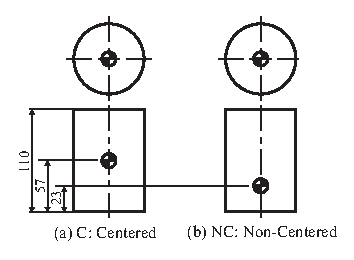
\includegraphics[width=0.3\textwidth]{figure/method/cylinder-property.eps}
 \caption{Manipulated cylinders.} 
 \label{fig:cylinder}
\end{figure}

\begin{table}[t!]
 \centering
 \caption{Specifications of the cylinders.}
      \begin{tabular}{|r||l|l|} \hline
               & Manipulation C & Manipulation NC \\ \hline \hline
              Weight & 455 g & 322 g \\ \hline
              Height & 110 mm & 110 mm \\ \hline
              Height of center of gravity & 57 mm & 23 mm \\ \hline
              Diameter & 72 mm & 72 mm \\ \hline
            \end{tabular}
    \label{tab:specification-of-robot}
\end{table}


% 実験風景
\begin{figure}[t!]
  \centering
  \includegraphics[width=0.45\textwidth]{figure/method/experiment-overview.eps}
  \caption{Overview of in-hand manipulation measurement. (A) Overview of experiment. (B) Reconstructed hand state using tactile data glove and motion capture system.}
 \label{fig:experiment-overview}
\end{figure}

% 操作??EスナップショチE??
\begin{figure*}[t!]
  \centering
  \includegraphics[width=0.98\textwidth]{figure/method/snapshot-m1.eps}
 \caption{Snapshots of rotating manipulation. Images of A--E represent the corresponding regrasping procedure.}
 \label{fig:snapshot}
\end{figure*}



\subsection{Identical Regrasping Procedure in In-hand Manipulation}

We observed the identical regrasping procedure in both manipulation C and NC (\figref{fig:snapshot}). Observed regrasping procedure is the following:
\begin{itemize}
    \item[A.] Put the index finger and the fingers from middle to little on the object
    \item[B.] Put the index finger to the object immediately after rotating the object
    \item[C.] Release and stretch the fingers from middle to little.
    \item[D.] Regrasp the object with all fingers
    \item[E.] Bend a thumb and put it to the object
\end{itemize}

\begin{figure*}[t!]
% 図: 抽出された接触運動
 \centering
  \includegraphics[width=.98\textwidth]{figure/experiment/m-db-ext.eps}
  \caption{Representative raster plots and mean active rate of PTP and non-PTPs from manipulations C and NC. Red points denote PTPs. Gray points denote non-PTPs. Blue solid line represents mean active rate of PTPs. Blue dashed line represents the mean active rate of all tactile points.}
 \label{fig:m-db-ext}
\end{figure*}

\subsection{Result}
%?E???E体的に英語??E記述の意味がわからなぁE????E忁E??結果なのにわからなぁE?Eは致命皁E??長、E??拙い表現で説明せず,定義した量??Eグラフ??E検定などチE?Eタに依ってごく簡潔??E瞭に結果を提示すべき!E
We characterized manipulations C and NC respectively, particularly addressing the numbers, spatial distributions and temporal distributions of PTPs and PMs.  First, the number of PTPs was 99 in manipulation C and 186 in manipulation NC. Similarly, the number of PMs was 2 in manipulation C and 12 in manipulation NC (\figref{fig:comp-tac}B, \figref{fig:comp-mot}). This shows that the in-hand manipulations were characterized not by all tactile points and motions but by partial ones, PTPs and PMs. Second, both PTPs from manipulation C and NC were localized from the thumb to the ring finger and from the palm near a thumb (\figref{fig:tac-dist}). Moreover, The PMs from manipulation C were localized in motions of a thumb (\figref{fig:comp-mot}(a)). The PMs from manipulation NC were also localized in motions of the fingers except for the index finger (\figref{fig:comp-mot}). Therefore spatial distributions of PTPs and PMs were found to be localized. Third, the representative segment shows that the PTPs from manipulation NC are localized in three time sections and the PTPs from manipulation C are localized in two time sections (\figref{fig:m-db-ext}). In addition, the PMs from manipulation C and NC were localized along the time-axis (\figref{fig:comp-mot}). We therefore found that the temporal distribution of PTPs and PMs were localized.

% 図: 運動の比輁E
\begin{figure}[t!]
 \centering
  \includegraphics[width=.48\textwidth]{figure/experiment/mot-comp-with-cap.eps} %{figure/final/motion-time-distribution-trial-1_2.eps} 
 \caption{Temporal distribution of PMs from manipulations of C and NC.}
 \label{fig:comp-mot}
\end{figure}


\begin{figure}[t!]
 \centering
  \includegraphics[width=.48\textwidth]{figure/experiment/tac-distribution.eps}
  \caption{Spatial distribution of PTPs from manipulations C and NC: (A) Spatial distribution of manipulation C. (B) Spatial distribution of manipulation NC.}
 \label{fig:tac-dist}
\end{figure}

% 刁E??付きの空間比輁E
% TODO figure not yet
\begin{figure*}[t!]
 \centering
  \includegraphics[width=.98\textwidth]{figure/experiment/temporal-tactile-points-with-variance.eps}
%  \includegraphics[width=.48\textwidth]{figure/experiment/temporal-tactile-points-with-variance.eps}
  \caption{Spatiotemporal distribution of PTPs at each section. (A and B) The average over trials of the mean active rate of the tactile points in manipulation C and NC. The red solid line and envelope show the average and variance of the mean active rate of PTPs over trials. The black solid line and envelope show the average and variance of the mean active rate of all tactile points over trials. (C--E) Spatial distribution of PTPs extracted from manipulation C at each section. (F--H) Spatial distribution of PTPs extracted from manipulation NC at each section. Circles in G and H show extracted differences of PTP patterns between manipulation C and NC.}
 \label{fig:temporal-tactile-points-with-variance}
\end{figure*}



To elucidate the differences of PTPs and PMs between manipulation C and NC, we compared manipulation C and NC, particularly addressing the share of spatial distributions and temporal distributions. First, the PTPs extracted from manipulation C shared 70\% (69 points) of these from manipulation NC (\figref{fig:comp-tac}B). The number of the PTPs only from NC was 117 points (11.5\% of the total) (\figref{comp-tac}(B)). In addition, all the PMs from manipulation C were extracted from manipulation NC (\figref{fig:comp-mot}), which suggests that there are common and task-specific PTPs and PMs. Second, three sections defined by local minima of all tactile points were found (\figref{fig:temporal-tactile-points-with-variance}). In the third section, the PTPs were found only from manipulation NC (see blue sections in \figref{fig:temporal-tactile-points-with-variance}AB). Therefore the temporal differences of PTPs were localized in a specific section. Third, visualizing the spatial distribution of the PTPs in each section, we found two spatial differences: On the one hand, PTPs in the middle finger and ring finger differed in the third section (\figref{fig:temporal-tactile-points-with-variance}EH). On the other hand, PTPs in the pulp of the index finger differed in the second section (\figref{fig:temporal-tactile-points-with-variance}DG). Thus, we found spatiotemporally localized specific differences of PTPs and PMs.

% 図: 接触運動の匁E??関俁E
\begin{figure}[!t]
 \centering
  \includegraphics[width=0.48\textwidth]{figure/experiment/comp-tac-with-cap.eps}
  \caption{Share relation between PTPs in manipulation C and manipulation NC. (A) Spatial distribution of PTPs in manipulation C and NC. Light red points represent PTPs in manipulations both C and NC, blue points only from manipulation C, and dark red from only from manipulation NC. (B) A Venn diagram of PTPs from manipulations C and NC.}
 \label{fig:comp-tac}
\end{figure}



%%%%%%%%%%%%%%%%%%%%%%%%%%%%%%%%%%%%%%%%%%%%%%%%%%%%%%%%%%%%%%%%%%%%%%%%%%%%%%%%
\section{Conclusion and Discussion}
% conclusion
The precise tactile points (PTPs) and precise motions (PMs) from a rotating cylinder manipulation were extracted using a data glove with high spatiotemporal resolution and analyses to select tactile-motion variables, particularly addressing precision. The PTPs were selected such that tactile points were active with high repeatability over trials. Their active timings have low variance. In addition, the PMs are selected such that motions appear with high repeatability over trials and their timings have low variance. Results show that PTPs and PMs are localized both spatially in the hand and temporally in the task. Moreover, we compared patterns of PTPs and PMs extracted by two manipulations of cylinders with different centers of mass, using identical regrasping procedures. We therefore suggest that patterns of PTPs and PMs characterize the precise difference of manipulations that are not distinguishable using earlier analytical methods.

% 重要だと言われてぁE??が,その方法??E確立してぁE??ぁE??E
% 手で初めて正確な状態を抽出?E?起き上がり??EコチE??似てぁE???E?従って?E?in-hand manipulationに新たな允E
Although control for dextrous manipulation with a robot hand persists as an important open problem\cite{bicchi2000hands}, no realistic controller has been developed. However, dynamic whole-body actions including complex contacts with the ground, for example roll-and-rise tasks, are known to have a "knack," an extremely narrow region in state-space to succeed\cite{kuniyoshi2007emergence}. The knacks are extracted by measuring human roll-and-rise tasks based on the convergence of the variance of motion trajectories. Emphasizing the knacks extracted from human measurement, an actual adult-size humanoid robot performs roll-and-rise motion\cite{kuniyoshi2004dynamic}. Similar to dynamic whole-body actions, we infer that PTPs and PMs extracted from human in-hand manipulation enable control of robotic in-hand manipulation.

% 難易度
We show that human hands adapt to more difficult manipulation by adding PTP patterns. Manipulation NC is more difficult than manipulation C because the center of gravity of the cylinder used in manipulation NC is closer to the edge of the supporting hand polygon than manipulation C. Focusing on the difference of PTP patterns, additional spatiotemporal patterns are extracted only from manipulation NC. This result implies that more difficult tasks necessitate the use of additional TPT patterns to stabilize the manipulation.

% 今後(網羁E??調査?E?ダイナミチE??なマニピュレーションの拘束条件としてロボット??E構??E?E?E
In future work, we will conduct experiments to extract precise tactile-motion patterns from other in-hand manipulations. Over the longer term, we plan to construct a robot controller using precise tactile-motor patterns extracted from human in-hand manipulation.
\addtolength{\textheight}{-12cm}   % This command serves to balance the column lengths
                                  % on the last page of the document manually. It shortens
                                  % the textheight of the last page by a suitable amount.
                                  % This command does not take effect until the next page
                                  % so it should come on the page before the last. Make
                                  % sure that you do not shorten the textheight too much.


%%%%%%%%%%%%%%%%%%%%%%%%%%%%%%%%%%%%%%%%%%%%%%%%%%%%%%%%%%%%%%%%%%%%%%%%%%%%%%%%
\section*{ACKNOWLEDGMENTS}
This work has been supported in part by JSPS Grant-in-Aid for Scientific Research(A) 26240039.

%%%%%%%%%%%%%%%%%%%%%%%%%%%%%%%%%%%%%%%%%%%%%%%%%%%%%%%%%%%%%%%%%%%%%%%%%%%%%%%%

%\begin{thebibliography}{99}
%\bibitem{c1} G. O. Young, Synthetic structure of industrial plastics (Book style with paper title and editor), in Plastics, Second ed. vol. 3, J. Peters, Ed.  New York: McGraw-Hill, 1964, pp. 1564.
%\end{thebibliography}



\bibliographystyle{IEEEtranS}
%\bibliographystyle{junsrt}
\bibliography{bibTeX/thesis}



\end{document}
